\section{Introduction}\label{sec:intro}

\begin{figure}
  \centering
  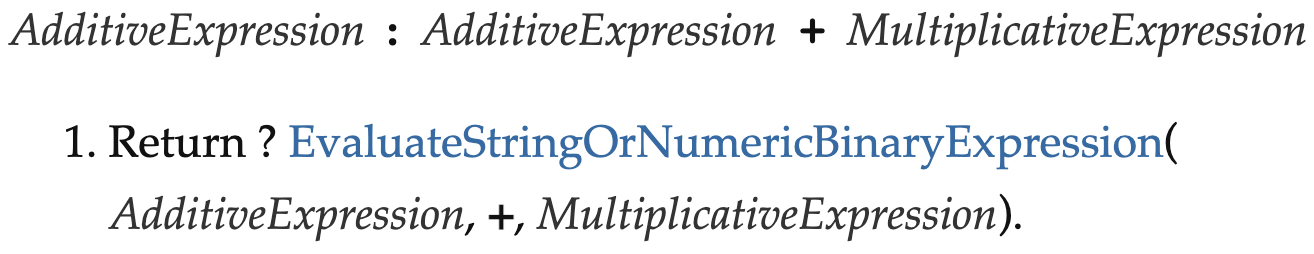
\includegraphics[width=\columnwidth]{img/add-eval.png}
  \caption{The \esalg{Evaluation} algorithm of the addition operator
  ($\code{+}$) in ES12}
  \vspace*{-1em}
  \label{fig:add-eval}
\end{figure}

In the beginning, JavaScript was a simple scripting language designed in a
ten-day hack. However, it has become a de facto Web standard and eventually
became one of the dominating programming languages in various fields. For
example, Node.js~\cite{nodejs} introduced full-stack JavaScript by supporting
server-side programming.  In addition, React Native~\cite{react-native} provides
a way to deploy JavaScript programs as mobile and desktop applications even
running on different platforms.  Furthermore, according to the annual report of
GitHub, JavaScript has consistently been the most popular programming language
based on the number of contributors to GitHub
projects.\footnote{\url{https://octoverse.github.com/}}

However, despite its popularity, developers and even JavaScript experts often
suffer from its highly dynamic nature.  JavaScript supports diverse dynamic and
complex language features, including higher-order functions, property accessors
with accessors, mutable prototypes chain, and asynchronous functions.  For
instance, the addition operator is not commutative, and even its result type
might be dependent on the order of the operands as follows:
\begin{center}
  \begin{tabular}{c}
    \begin{lstlisting}[style=JS]
{} + "" // 0
"" + {} // "[object Object]"
    \end{lstlisting}
  \end{tabular}
\end{center}
The result of the addition between an empty object $\;\jscode{\{\}}$ and an empty
string $\jscode{""}$ is a number $\jscode{0}$, but it becomes a string
$\jscode{"[object Object]"}$ with the reversed order of operands.  It happens
because the addition operator has complex rules for implicit type conversions in
JavaScript while it simply represents numeric additions or string concatenation
in most other languages.  Such a dynamic nature of JavaScript causes pain to
developers in understanding the language semantics.  Besides, it is challenging
to understand the detailed semantics even for the JavaScript experts.  For
example, while V8 is the most widely-used JavaScript engine developed by Google
for Node.js and Chrome web browsers, its semantic bugs have consistently been
reported to its issue tracker.\footnote{\url{https://bugs.chromium.org/p/v8}}

Therefore, when they desire to understand the detailed semantics of JavaScript,
they refer to \textit{ECMA-262}.  It is the standard specification written in
English defining ECMAScript, which is the official name of JavaScript.  It
describes the syntax via a variant of the extended Backus–Naur form and the
semantics via abstract algorithms consisting of structured steps.  For example,
Figure~\ref{fig:add-eval} shows the \esalg{Evaluation} algorithm of the addition
operator in the latest ECMA-262 (ES12, 2021)~\cite{es12}.
\footnote{\url{https://262.ecma-international.org/12.0/\#sec-addition-operator-plus}}
It consists of a single step that invokes another algorithm,
\esalg{EvaluateStringOrNumericBinaryExpression}; the first and third arguments
are the left and right subtrees of the abstract syntax tree (AST) for a given
additive expression, and the second one is a text \code{+} to represent the
additive operation.  The \esalg{EvaluateStringOrNumericBinaryExpression} is a
generic algorithm for string or numeric binary operations (e.g., \code{-},
\code{*}, \code{<}, etc.).

Unfortunately, it is still challenging to 1) understand all the \textit{possible
behaviors} of language features and 2) find \textit{example programs} that
trigger each behavior by only referring to the language specification.  First,
it is not an easy task to answer which behaviors are possible in language
features.  For example, a language feature in JavaScript often has unexpected
behaviors, such as implicit function calls, implicit property reads/writes, or
runtime exceptions with different typed errors.  Besides, the problem becomes
more complicated if we want to know possible behaviors of language features used
with specific types of values or other language features.  Second, even if users
realize a specific behavior of a language feature, it is nontrivial to find
example programs that trigger the behavior.  For instance, Assume that we
realize that the addition operator might cause implicit function calls.
However, we should make an additional effort to grasp when it is triggered if we
want to find example programs as follows:
\begin{center}
  \begin{tabular}{c}
    \begin{lstlisting}[style=JS]
var x = { toString: () => "a" };
x + "b"; // "ab" with an implicit call of `x.toString()`
    \end{lstlisting}
  \end{tabular}
\end{center}
In this code, the left and right operands have different types \code{Object} and
\code{String}, respectively.  It causes an implicit conversion from the object
in the variable \code{x} to a string value with an implicit call of the function
in \code{x.toString}.

To alleviate this problem, we present $\tool$, which automatically infers
possible behaviors of JavaScript language features from ECMA-262 and finds
corresponding example programs.  We first introduce \textit{syntactic views}, an
extension of a JavaScript abstract syntax tree (AST) consisting of both concrete
and abstract nodes with a type bound.  Users can freely construct syntactic
views depending on which semantics they want to understand; concrete nodes
denote the language features they want to understand, and abstract ones denote
the parts they do not.  Then, our tool reduces ECMA-262 to consist of only
abstract algorithms reachable from a given syntactic view.  Our key observation
is that the reachability of specific algorithms in the language specification
implies possible behaviors of language features.  For example, the \esalg{Call}
algorithm in ECMA-262 represents function calls.  Thus, if we want to know
whether the addition operator can cause implicit function calls, we should check
that it is reachable from the \esalg{Evaluation} algorithm of the addition
operator.  Finally, $\tool$ searches example programs in Test262~\cite{test262},
an official JavaScript conformance test suite, for each algorithm in the reduced
specification.  Our tool searches example programs in Test262 using program
execution traces on the specification collected before the search.  We evaluated
the effectiveness of $\tool$ with the latest ECMA-262 (ES12, 2021) and showed
its practicality with \inred{three} advanced syntactic views.

Our contributions are as follows:
\begin{itemize}
  \item We introduce a \textit{syntactic view}, an extension of a JavaScript
    abstract syntax tree (AST) consisting of both concrete and abstract nodes
    with a type bound, to help users indicate which language features they want
    to understand.

  \item We present an automatic way to 1) infer \textit{possible behaviors} of
    JavaScript language features by reducing ECMA-262 and checking the
    reachability of algorithms and 2) search \textit{example programs} in
    Test262 using program execution traces on the specification collected before
    the search.

  \item We actualize our techniques in $\tool$ and evaluate its effectiveness
    using the latest ECMA-262 with \inred{177} basic syntactic views and discuss
    its practicality with \inred{three} advanced syntactic views.
\end{itemize}
